\documentclass[11pt]{article}
\usepackage[T1]{fontenc}
\usepackage[utf8]{inputenc}
\usepackage{lmodern,microtype}
\usepackage{amsmath,amssymb,amsthm,mathtools}
\usepackage[a4paper,margin=25mm,headheight=14pt]{geometry}
\usepackage{booktabs,array,longtable}
\usepackage{tikz,fancyhdr}
\usepackage{xurl}
\usepackage[colorlinks=true,allcolors=blue!45!black]{hyperref}
\hypersetup{pdftitle={Certified rational-anchor filtering for exact GPU scans of power-residue runs},pdfauthor={Brice Pouly}}
\pagestyle{fancy}\fancyhf{}
\fancyhead[L]{\small Exact GPU scans of power-residue runs}
\fancyhead[R]{}\fancyfoot[C]{\thepage}
\renewcommand{\headrulewidth}{0.3pt}
\newtheorem{theorem}{Theorem}[section]
\newtheorem{proposition}[theorem]{Proposition}
\newtheorem{lemma}[theorem]{Lemma}
\theoremstyle{definition}\newtheorem{remark}[theorem]{Remark}
\newcommand{\Fp}{\mathbb F_p}
\newcommand{\Z}{\mathbb Z}
\newcommand{\cl}{c_r}
\newcommand{\data}{\texttt{results/gpu-algorithms/2026-10-02/}}
\newcolumntype{P}[1]{>{\raggedright\arraybackslash}p{#1}}
\title{Certified rational-anchor filtering\\
for exact GPU scans of power-residue runs}
\author{Brice Pouly\thanks{Prepared with artificial-intelligence assistance; see the declaration at the end.}}
\date{12 October 2026}
\hypersetup{pdfsubject={Publication edition v1.0; 12 October 2026}}
\begin{document}\maketitle
\begin{abstract}
We study exact longest monochromatic runs of power-residue colourings,
including neutral prefixes and least canonical witnesses. A certified
rational cover represents every relevant interval inside a short signed
character table. A reflection-compatible schedule retains an anchor;
conservative filters reject only known contradictions, bilateral completion
recovers the full run, and tie-preserving reduction selects its least
witness. We prove this exact-success contract and describe its CUDA
realization with separate arithmetic domains below $2^{32}$ and $2^{33}$.
On one RTX 5090, two reserved cohorts give ratios $24.00$ and $10.95$ of
sums of hot per-prime medians against the identified historical dense
engine. A separate batch study gives throughput factors $1.23$--$2.58$
against an already optimized reference. The experiments have different
timing boundaries and their factors are reported separately. Short-table
multiplicative extraction has close algorithmic antecedents in cryptanalysis;
our contribution is its certified organization for exhaustive maxima and
witnesses and its measured implementation. Square-root-sized cover
parameters do not give a general $O(\sqrt p)$ running-time bound.
\end{abstract}
\noindent\textbf{Keywords.} Multiplicative characters; monochromatic runs;
Rabung construction; rational approximation; CUDA; reproducible computation.

\section{Problem and contribution}
Rabung's construction uses power-residue colourings to produce lower bounds
for van der Waerden numbers~\cite{rabung}. A prime and a colour count encode
the colouring succinctly, but the finite conditions must still be checked.
Computing an exact run profile is therefore useful both for searching for
candidate certificates and for building an experimental census. Distributed
searches by Monroe provide an important computational predecessor~\cite{monroe,monroecode}.
The published certificates paper separates GPU discovery from
pointwise certificate verification~\cite{bounds}. The present paper treats
the scanner itself as the object of study. Its exactness theorem concerns
ordinary maxima, prefixes and canonical witnesses. The coverage proof and
controlled measurements establish this computational contract independently
of any census classification or limiting probability law.

\paragraph{Reading contract.}
A successful scan returns $(M_r,L_r,K_r,w_r)$: the largest ordinary run,
the neutral prefix, the Rabung boundary threshold and the least start of
a maximizing run. Section~\ref{sec:contract} fixes these conventions.
Sections~3--4 establish coverage and conservative selection; Sections~5--6
explain profile sharing and execution; Sections~7--8 distinguish timings
from implementation checks. Capacity refusal is a reported failure, not a
statement that long runs are absent.

The central difficulty is to reduce expensive character evaluations without
assuming that long runs behave randomly. A probabilistic estimate for a
typical maximum can guide experiments, but cannot justify discarding a
candidate in an exact scan. We instead construct a geometric hitting set:
every relevant interval has a rational representation with bounded numerator
and denominator; a short monochromatic anchor then identifies a candidate
whose maximal extent is reconstructed exactly.

The contributions developed here are an integer certificate for the cover,
a reflection-compatible anchor schedule, conservative bit filters, and an
implementation that retains exact maxima, prefixes and canonical witnesses.
The implementation combines adaptive warp partitioning, character-profile
sharing and concurrent streams, with explicit failures for resource or
domain violations. The measured gains have two distinct baselines: the
historical dense engine, and a later qualified sparse engine. This distinction
is essential to assessing the scale of the improvement.

Minkowski's theorem, multiplicativity, Montgomery reduction and CUDA streams
are established tools. Our claims concern their explicit assembly for this
finite scanning problem and the archived measurements. The article does not
claim priority for rational approximation or for any general-purpose GPU
technique. The related work below identifies close algorithmic precedents. We make no
claim that the primitives or their use for extracting sequences were invented
here, and no exhaustive priority claim for the complete assembly.

\paragraph{Scope.}
The experiments use every $r\in\{2,\ldots,9\}$ dividing $p-1$, rather than
only a fixed intersection of congruence classes. The optimized workers accept
prime inputs $1000\le p<2^{33}$, using distinct 32-bit and wider paths. Type
bounds do not promise successful execution for every input: table, seed and
queue guards may refuse a case. Small-prime handling belongs to a separate
exact preparation path. All measurements discussed here predate the completed atlas campaign.
The atlas and new numerical bounds retain their own evidence; dissemination and evidence limits
are collected in Section~\ref{sec:reproducibility}.

\subsection{Related work and the precise contribution}
First occurrences of power-residue runs were studied by Lehmer and Lehmer
and by Rabung and Jordan~\cite{lehmer,rabungjordan}. Buell and Hudson
computed longest quadratic-residue and nonresidue runs for primes below
420\,000~\cite{buell}. Their publisher's abstract and bibliography establish
that the observable and a census of maxima are older. Their full paper and
LSU report 83-017 were not obtained; their internal algorithm is therefore
not claimed to differ from ours in every respect.

Beullens, Beyne, Udovenko and Vitto~\cite{beullens}, Sections 3.2, 3.4 and
7.2, already exploit multiplicativity, arithmetic subsequences, denominators
and reversal to extract many normalized sequences from a short table, with
extensions to power-residue symbols. Their Section 3.1 also gives a
deterministic table-search variant. Kalu\dj erovi\'c, Kleinjung and
Kosti\'c~\cite{kkk}, Sections 3--5 and Appendix A, develop multiplicative
extraction, reuse, reversal and bit-matrix transposition. These are close
algorithmic precedents, rather than merely the same elementary identity.
Their key-recovery contract does not automatically supply exhaustive run
maxima and their canonical ties. Conversely, this different output contract
does not erase the precedent for the primitives. We cite the revised
ePrint text for these details; the related ANTS XIV article has a different
title~\cite{kkkants}.

Small modular representatives also belong to classical Thue and Euclidean
methods and rational reconstruction~\cite{shoup,wang}. Reconstruction seeks a
small fraction, often unique if it exists in a regime $2BD<p$; it can
legitimately report that none exists. Our clipped window condition implies
$BD>p$ and ensures existence for every relevant interval. Neither the
lattice principle nor rational normalization is new. The contribution
claimed here is the cover--hitting-set--conservative-filter--completion
composition with a stated output contract, not priority for its ingredients.

\begin{table}[ht]
\centering\small
\begin{tabular}{P{.24\textwidth}P{.31\textwidth}P{.37\textwidth}}
\toprule Predecessor & Work and output & Relation to this scanner\\\midrule
Buell--Hudson & Quadratic run maxima and census & Same kind of observable; internal algorithm not inspected.\\
Monroe paper/code & Full power table, shared orders, maximum/prefix/boundary threshold & Dense precedent; no per-position exponentiation is required to fill the table; no canonical witness exposed by the inspected code.\\
Beullens et al.; Kalu\dj erovi\'c et al. & Short-table extraction, reversal, bit operations for key recovery & Direct precedent for primitives; different output and coverage obligations.\\
Thue/reconstruction & Bounded modular representatives; uniqueness/conditional reconstruction & Classical foundations; whole-window existence is the role of our explicit certificate.\\
This work & Certified window cover, complete folded anchor set, safe rejection, exact completion & Exact $M_r,L_r,K_r,w_r$ on successful execution under the stated hypotheses.\\
\bottomrule
\end{tabular}
\caption{Algorithmic comparison, not a common-machine timing comparison or
an assertion of universal priority.}
\end{table}

\section{Exact output contract}\label{sec:contract}
Fix an odd prime $p$ and an admissible $r\ge2$. Choose a surjective additive
label for a multiplicative character of order $r$,
\[
 \cl:\Fp^{\times}\longrightarrow\Z/r\Z,
 \qquad \cl(xy)=\cl(x)+\cl(y).
\]
For a primitive root $g$, one choice is $\cl(g^j)=j\bmod r$. The kernel
is the subgroup of $r$th powers; the choice of labels permutes the colours
and has no effect on equality of colours. We scan the ordinary integer
sequence $1,\ldots,p-1$. Zero is excluded, and an interval does not wrap
cyclically through it.

Let $M_r$ be the largest length of a constant-colour interval, and let $L_r$
be the longest initial interval with colour zero. Thus $L_r\ge1$, since
$\cl(1)=0$. For a maximal run $[l,h]$, its reflected partner is
$[p-h,p-l]$, because
\begin{equation}\label{eq:reflection}
 \cl(p-x)=\cl(x)+\sigma_r,\qquad
 \sigma_r=\cl(-1)=\frac{p-1}{2}\bmod r.
\end{equation}
The canonical witness is the least start among all runs of length $M_r$;
reflection allows each pair to contribute $\min(l,p-h)$. A tie is part of
the output contract, not a dispensable side effect of finding the maximum.

The scanner also reports
\begin{equation}\label{eq:K}
 K_r=\max\{M_r+1,\, B_r\},\qquad
 B_r=\begin{cases}
 2L_r+2,&r\mid(p-1)/2,\\
 L_r+2,&r\nmid(p-1)/2.
 \end{cases}
\end{equation}
Here $B_r$ is a boundary threshold and is unrelated to the table radius
$B$ used below. Criterion (a) for a requested length $k$ checks $p>k$ and
$M_r<k$; the combined criterion (a)+(b) checks $p>k$ and $K_r\le k$.
These conditions describe distinct outputs. A fast scan of criterion (a)
alone is not automatically a certificate for the combined condition.
We use colour-first notation $W(r,k)$, with $r$ colours and progression
length $k$, as in the published certificates paper~\cite{bounds}.
That paper proves the boundary-test equivalence and owns the numerical
bound comparisons. The present output contract supports those applications;
no new lower-bound theorem is announced here.

\subsection{Dense reference}
The historical CUDA engine evaluates the character across a half interval
and uses~\eqref{eq:reflection} to recover the full profile. It fuses
admissible character orders using their least common multiple. Consecutive
segments retain their endpoint colours, prefix, suffix and internal maximum;
an ordered associative merge reconstructs boundary-crossing runs. When the
central colours match, the central junction is merged explicitly.
The baseline therefore already exploits symmetry, parallelism and shared
character evaluation. Comparing against it is more informative than
comparing with a naive serial scan.

Monroe's inspected \texttt{uc2.cpp} builds a common discrete-log table by
successive multiplication of a primitive root, then scans its entries for
several orders~\cite{monroecode}. Filling it takes $O(p)$ modular
multiplications and $\Theta(p)$ stored labels after root preparation; the
pass across a fixed set of orders is linear. Thus a dense method need not
perform one exponentiation per position. The historical CUDA baseline here
instead trades dense storage for character evaluation over the half
interval. Its small root-image table has at most 2520 entries. Our sparse
engine prepares $O(B)$ character values, visits scheduled words and
completes survivors. These are different work/memory tradeoffs; no timing
factor against Monroe is available. Sharing orders and the boundary
formula are also present in that earlier software, not introduced here.

\subsection{A root of the required order}
Let $\mathcal R$ be the requested orders and $m=\operatorname{lcm}\mathcal R$.
For the admissible subset of $2,\ldots,9$, $m\le2520$ and $m\mid p-1$.
To tabulate the image of $x\mapsto x^{(p-1)/m}$, it suffices to find an
element $z$ of order exactly $m$. Trial values
$z=a^{(p-1)/m}$ are accepted if
\[
 z^{m/q}\ne1\quad\hbox{for each prime }q\mid m.
\]
Only the small integer $m$ must be factored; a primitive root of order $p-1$
is unnecessary. The case $m=2$ uses $z=-1$. Any two choices of $z$ differ by
a power $u$ invertible modulo $m$. The resulting relabelling preserves
colour equality, the zero prefix, subgroup refinements and~\eqref{eq:reflection}.
This optimization does not compute an unrestricted discrete logarithm.

\section{Certified rational covers}\label{sec:cover}
Multiplicativity gives
\begin{equation}\label{eq:quotient}
 \cl(a/d)=\cl(a)-\cl(d)
 \quad(a,d\ne0\bmod p).
\end{equation}
Consequently, if an interval admits representatives
$a,a+d,\ldots,a+(Q-1)d$ in a short signed table, testing its colours requires
table comparisons instead of one modular exponentiation per position.
The following certificate guarantees such a representation. It is an
application of the classical convex-body theorem~\cite{minkowski}.
The short-table use of~\eqref{eq:quotient} has algorithmic precedents in
cryptanalysis~\cite{beullens,kkk}; the certificate supplies the exhaustive
window guarantee needed for our distinct output contract.

\begin{theorem}[Integer coverage certificate]\label{thm:cover}
Let $3\le Q\le p-1$, $H=Q-1$, and let positive integers $B,D$ satisfy
\begin{equation}\label{eq:certificate}
 B<p,\quad D<p,\quad HD\le2B,\quad 4BD-HD^2>4p.
\end{equation}
For every interval $x,x+1,\ldots,x+H$ in $\{1,\ldots,p-1\}$, there are
integers $a,d$ with $1\le d\le D$, $\gcd(a,d)=1$ and
\[
 a\equiv dx\pmod p,\qquad |a+jd|\le B\quad(0\le j\le H).
\]
None of these numerators is zero.
\end{theorem}
\begin{proof}
The lattice
\[
 \Lambda_x=\{(a,d)\in\Z^2:a\equiv dx\pmod p\}
\]
has basis $(p,0),(x,1)$ and determinant $p$. Apply the determinant-one
shear $(a,d)\mapsto(A,d)=(a+Hd/2,d)$. In these coordinates the centrally
symmetric convex body
\[
 \mathcal C=\{(A,d):|d|\le D,\ |A|+H|d|/2\le B\}
\]
has area
\[
 \int_{-D}^{D}(2B-H|d|)\,\mathrm d d=4BD-HD^2>4p.
\]
Minkowski's theorem supplies a nonzero lattice point. If $d=0$, then
$a$ is a nonzero multiple of $p$ with $|a|\le B<p$, a contradiction.
Change sign so that $d>0$. The convex-body inequality bounds both endpoints
$a$ and $a+Hd$ by $B$ in absolute value, hence every intermediate numerator.
If $s=\gcd(a,d)>1$, divide both coordinates by $s$. Since $s\le d<p$,
$s$ is invertible modulo $p$; the congruence is preserved and the bounds
only decrease. Finally, $a+jd\equiv d(x+j)\not\equiv0\pmod p$, so no
numerator can equal zero.
\end{proof}

The shear can have half-integer coordinates when $H$ is odd. It still maps
the lattice by a real linear transformation of determinant one, so its
covolume is unchanged. There is no rounding step in the proof.
For an interval of length $q\le Q$, extend it to a $Q$-interval inside
$\{1,\ldots,p-1\}$, when $Q\le p-1$, and restrict the representation.
Thus the same certificate covers all shorter thresholds.

\paragraph{A complete small example.}
For $p=101$, $r=2$, $Q=q=5$, $H=4$, $D=4$ and $B=30$, the
integer certificate is $HD=16\le60$ and
$4BD-HD^2=416>404=4p$. The window $19,\ldots,23$ has numerator
row $-25,-21,-17,-13,-9$, since $-25+4j\equiv4(19+j)\pmod{101}$.
Multiplicativity reads its colours in the signed table after subtracting
the common label of $4$. With $t=3$, spacing $s=q-t+1=3$ and phase
$\phi=1$, the folded anchor has $b=17=4\cdot4+1$: its quotient
$n=4$ satisfies $n\equiv1\pmod3$. Completion uses
$x=-17\cdot4^{-1}=21\pmod{101}$ and recovers $[19,25]$.
Its reflected partner is $[76,82]$, so its canonical start is $19$.
A literal character scan gives $(M_2,L_2,K_2,w_2)=(7,1,8,19)$.
This arithmetic example illustrates the cover, selection and completion;
it is below the optimized workers' accepted range and is not a GPU timing
or an additional qualification input.

\subsection{Choosing parameters without trusting floating point}
On the branch $HD^2\le4p$, the least table radius satisfying the strict
area inequality is
\begin{equation}\label{eq:Bchoice}
 B=\left\lfloor\frac{4p+HD^2}{4D}\right\rfloor+1.
\end{equation}
The branch condition also ensures $HD\le2B$. The implementation checks all
of~\eqref{eq:certificate} using integer arithmetic after choosing parameters;
a rounded square root can propose a candidate, but cannot certify it.
Table capacities and signed filter indices impose additional guards.

Ignoring integer rounding, let $D_0=2\sqrt{p/H}$ and choose $D=D_0/n$.
Then the area boundary gives
\begin{equation}\label{eq:volume}
 B\simeq\sqrt{Hp}\left(\frac n2+\frac1{2n}\right),\qquad
 BD\simeq p(1+n^{-2}).
\end{equation}
Changing $n=2$ to $n=4$ reduces this rectangle proxy from $1.25p$ to
$1.0625p$, while increasing the table radius. Larger tables put additional
pressure on cache and shared memory. This is an architectural tradeoff,
not a theorem that larger $n$ is always faster.

\begin{figure}[ht]
\centering
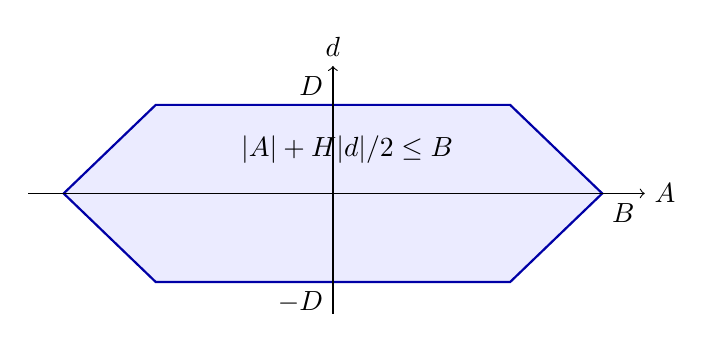
\begin{tikzpicture}[scale=0.9]
 \fill[blue!8] (-2.5,-1.25)--(2.5,-1.25)--(3.8,0)--(2.5,1.25)--(-2.5,1.25)--(-3.8,0)--cycle;
 \draw[blue!65!black,thick] (-2.5,-1.25)--(2.5,-1.25)--(3.8,0)--(2.5,1.25)--(-2.5,1.25)--(-3.8,0)--cycle;
 \draw[->](-4.3,0)--(4.4,0) node[right]{$A$};
 \draw[->](0,-1.7)--(0,1.8) node[above]{$d$};
 \node[below right] at (3.8,0){$B$};
 \node[above left] at (0,1.25){$D$};
 \node[below left] at (0,-1.25){$-D$};
 \node at (0.2,0.62){$|A|+H|d|/2\le B$};
\end{tikzpicture}
\caption{The symmetric clipped cover in sheared coordinates. Its area is
$4BD-HD^2$. The diagram illustrates the certificate, not a measured work count.}
\label{fig:cover}
\end{figure}

\section{Anchors, conservative rejection and exact completion}\label{sec:anchors}
The cover supplies a bounded arithmetic progression of numerators for any
run worth retaining. The implementation enumerates short anchors from this
representation, filters them in words of 32 candidate bits, and extends the
survivors to their true boundaries in the original sequence.

\subsection{A reflection-compatible hitting set}
Suppose a run contains a $q$-window and $3\le t\le q$. There are
$s=q-t+1$ possible starts for a $t$-anchor within that window. Along a
rational row these starts have numerators differing by $d$. A periodic
selection with period $s$ therefore hits at least one of them.
The signed table is folded using reflection. It is useful to make the
selection commute with that fold, rather than relying on a favourable
location of the run.

\begin{lemma}[Symmetric anchor schedule]\label{lem:schedule}
For the increasing representation $a,a+d,\ldots,a+(t-1)d$, define
$b=a+(t-1)d$. The same anchor, in descending order, is
$(b,b-d,\ldots,b-(t-1)d)$. Negating and reversing it sends its first
numerator to $(t-1)d-b$. For $d>2$ and a primitive pair $(b,d)$, write
$b=nd+c$, $0<c<d$, using Euclidean division even if $b$ is signed.
Choose any phase $\phi\in\{0,\ldots,s-1\}$, and select $b$ if
\begin{equation}\label{eq:schedule}
 n\equiv\begin{cases}
 \phi,&2c<d,\\
 t-2-\phi,&2c>d
 \end{cases}\pmod s.
\end{equation}
Selection is invariant under $b\mapsto(t-1)d-b$. Every $q$-window in a
primitive rational row contains a selected $t$-anchor, whose orientation
may be chosen to satisfy $b\ge(t-1)d/2$. For $d=1,2$, retaining all
starts has the same hitting property.
\end{lemma}
\begin{proof}
Reflection replaces $n$ by $t-2-n$ and $c$ by $d-c$, which exchanges the
two branches of~\eqref{eq:schedule}. The cases $c=0$ and $2c=d$ cannot
occur in a primitive pair with $d>2$. Within the $q$-window the $s$
possible starts have one fixed nonzero residue $c$ and $s$ consecutive
quotients $n$, so exactly one satisfies the appropriate congruence.
If its centre is negative, reflection makes it nonnegative and preserves
selection. All reflected numerators retain their absolute table bounds.
\end{proof}

After the fold, the enumeration domain is
\begin{equation}\label{eq:folded}
 1\le d\le D,\qquad
 \left\lceil\frac{(t-1)d}{2}\right\rceil\le b\le B,
 \qquad\gcd(b,d)=1.
\end{equation}
The span $(t-1)d\le HD\le2B$ ensures that all anchor numerators lie in
the signed table. Zero numerators are excluded. The right endpoint of the
unreflected anchor is $bd^{-1}\bmod p$; the completion code uses the
reflected increasing anchor beginning at $x=-bd^{-1}\bmod p$, with
numerators $-b+jd$. It checks $x\ne0$ and $x+t\le p$, so it never treats a
zero-crossing cyclic interval as a run.

In \texttt{periodic\_bands.hpp}, a band has $b=nd+c$ with
$1\le c<d/2$ or $d/2<c\le d-1$, clipped to~\eqref{eq:folded}.
The complementary phase is $(t-2-\phi)\bmod s$. The retained kernels use
one phase $\phi=\lfloor(t-1)/2\rfloor\bmod s$ for the whole denominator
row in an epoch, not independent phases for adjacent bands. The wheel
$G=\gcd(d,6)$ restricts to $b\equiv c_G\pmod G$: one row for $G=1,2$,
two rows for $G=3,6$. Additional masks can remove some nonprimitive pairs;
the exact gcd check occurs in completion. A primitive pair is never removed.
For $d=1,2$ all primitive starts are retained.
Ranks enumerate the first clipped band, the translated interior bands and
the last clipped band; \texttt{floor\_div}/\texttt{ceil\_div} explicitly
handle signed endpoints. Colour values do not change this partition.

\paragraph{Total policy for anchor length (retained mode 13).}
The implementation is \texttt{anchor\_t} in \texttt{gpu\_pipeline.cuh}.
For $q\ge3$ put
\[
 h=\lceil q/2\rceil,\quad s_0=q-h+1,\quad
 u=2^{\lfloor\log_2s_0\rfloor},\quad v=q-u+1.
\]
Set $z=v$ only if $h\le v\le h+2$; otherwise set $z=h$. Return
$t_{\rm proposed}=\min(q,\max(3,z))$. The selected 32-bit worker chooses
it at seed completion and keeps that $t$ for later epochs; its $q_e$ can
still increase. The selected wider worker enables dynamic anchor length:
a later epoch uses $t_e=\max(t_{e-1},t_{\rm proposed})$. Verified maxima
and thus $q_e$ are nondecreasing. Both policies preserve $3\le t_e\le q_e$.
For $q=12$ the proposal $v=9$ is rejected, yielding $t=6,s=7$; for
$q=13$, $v=10$ is rejected, yielding $t=7,s=7$. Power-of-two spacing is
an optional optimization with a general-period fallback, not a universal
promise within two increments. The finite revision check covers every
$3\le q\le256$ and the monotone epoch invariant without running CUDA.
Completion can return a run much longer than $Q$.


\subsection{What a bit filter is allowed to reject}
For each character bit plane, aligned table words are compared at the
offsets of an anchor. A candidate survives only when all its known anchor
colours agree. Quotienting by $d$ changes each label by the same constant,
so equality of numerator colours is sufficient. A wheel can omit pairs
whose common divisor prevents them being primitive. A skipped residue
must be excluded arithmetically, not because it looks unlikely.

Entries outside the table are unknown. They do not count as a mismatch.
This convention is essential near clipped boundaries and when the
completion extends beyond the representation certified by the short window.

\begin{lemma}[Bilateral rejection]\label{lem:cuts}
Consider a constant-colour anchor of length $t$. Suppose a different known
colour is observed $i\ge1$ places to the left of its first position and
$j\ge1$ places to the right of its last position. The run containing the
anchor has length at most $t+i+j-2$. In particular, if both mismatches are
found within budgets $U,V$ with $U+V\le q-t+1$, that run has length less
than $q$.
\end{lemma}
\begin{proof}
The run can include at most $i-1$ additional positions on the left and
$j-1$ on the right. For the budget statement, its length is at most
$t+U+V-2\le q-1$.
\end{proof}

This lemma explains a simple two-cut filter. The retained mode is stronger:
it considers every placement of a $q$-window containing the anchor, and
keeps a candidate if at least one placement has no known mismatch. An
actual run of length at least $q$ supplies such a placement, so rejecting
all placements is safe. The implementation performs this screen only when
$q-t\le32$; otherwise it retains the candidate. Its mode-four guard is
\texttt{h>32}, with a 33-element array for positions $0,\ldots,32$;
this path does not shift a 32-bit word by 32. Neither filter assumes that
the anchor starts at the head of a maximal run.

\subsection{Thresholds and canonical ties}
A pilot establishes a real monochromatic run and hence a lower bound for
the maximum. Each denominator epoch takes a snapshot of this bound and
caps its geometric threshold by $Q$. For a coupled pair of profiles, the
shared search uses a threshold no larger than either current maximum.
The threshold stays immutable throughout the generation and completion
kernels of that epoch; it is updated only after ordered completion.

To retain the least witness, the search must preserve anchors in runs whose
length equals the current maximum. It may reject runs certified to be
strictly shorter. At completion, each surviving anchor is mapped to a
position of the original sequence using~\eqref{eq:quotient}, extended in
both directions, and reduced by length and then by least canonical start.
The prefix is checked directly using modular powers. If the pilot cannot
establish the required threshold, or a queue overflows, the engine produces
a failure rather than an approximate maximum.

The geometric certificate, the hitting-set argument and conservative
rejection explain why a relevant run is retained at the algorithmic level.
Correctness of its CUDA realization additionally depends on the finite
partition, synchronization, arithmetic and output checks described below.
A test passing does not replace a proof of the cover, and a proof of the
cover does not verify an arbitrary CUDA implementation.

\subsection{Composition into an exact-success contract}\label{sec:global}
Consider a true global maximum. Its covering denominator is assigned to one
epoch. The verified maximum available at that epoch gives a threshold no
larger than the true maximum, so a subwindow at that threshold contains a
scheduled anchor. Known contradictions cannot eliminate that anchor.
Exact completion recovers the run, and the tie rule keeps its least start.
Later increases in the threshold do not require revisiting earlier epochs.
The theorem states precisely the implementation hypotheses for this argument.
\begin{theorem}[Exactness on successful termination]\label{thm:global}
For each profile $r$, fix $(B,D,Q)$ satisfying
Theorem~\ref{thm:cover}, with $3\le Q\le p-1$. Suppose disjoint denominator
epochs exhaust $\{1,\ldots,D\}$. In epoch $e$, use a fixed threshold
\[
 3\le q_e\le\min(Q,m_{r,e})\le\min(Q,M_r),
\]
where $m_{r,e}$ is the length of a run verified before that epoch, and use
$3\le t_e\le q_e$. Suppose enumeration preserves the complete scheduled
primitive anchor set, modulo reflection; rejection is conservative for
each profile; completion and colour arithmetic are exact; and each
surviving obligation is completed to its true boundaries without passing
zero. Assume no lost task, capacity overflow, failed arithmetic guard or
unfinished epoch is accepted as success. Then reduction by length and
least canonical start returns $M_r,w_r$. An exact prefix check returns
$L_r$, and~\eqref{eq:K} returns $K_r$.
For coupled profiles these assumptions apply to each profile separately;
candidate routing must preserve their union of obligations.
\end{theorem}
\begin{proof}
Verified seed and completed runs have length at most $M_r$. Fix any
maximum run and a subwindow $J$ of length $\min(M_r,Q)$. Extend $J$ to
a $Q$-window within $1,\ldots,p-1$ if necessary. The cover gives a
primitive representation with some $d\le D$; restriction preserves its
primitivity and table bounds. That denominator belongs to an epoch $e$.
Because $q_e\le |J|$, a $q_e$-subwindow contains a scheduled $t_e$-anchor.
Reflection may place it in the reflected run of the same length.
An actual monochromatic window has no observed contradiction, so a
conservative profile filter retains its obligation. Exact completion finds
the maximum run or its partner. This holds for every maximum run, so the
reduction also finds the least start among ties. Completion produces only
real runs, excluding an overestimate. Direct prefix verification and the
integer formula give the remaining outputs.
\end{proof}

\noindent\textbf{Algorithm 1 (logical specification; each failure is visible).}
\begin{enumerate}
\setlength{\itemsep}{1pt}
\item Validate input, arithmetic and capacities; certify fixed group covers;
prepare signed character planes and inverses.
\item Establish real seed runs and their canonicalized witnesses. Refuse
if the required threshold cannot be established.
\item For each denominator epoch, snapshot per-profile maxima, choose
$q_e,t_e$, and build whole-row folded plans.
\item Generate primitive anchor words; test coarse anchors and maintain
separate profile obligations. Reject only under the appropriate profile's
known contradictions. Queue a word if any obligation remains.
\item Complete queued obligations and reduce maxima/ties; check queue
counts, errors, dependencies and epoch completion before advancing.
\item Verify witnesses and prefixes, form $K_r$, and report success only
after all epochs for all requested groups have completed.
\end{enumerate}
The theorem specifies the algorithm's mathematical contract. It is not a
formal verification of CUDA instructions, binary identity or the absence
of every software defect. Evidence for those implementation bridges is
recorded separately in Section~\ref{sec:verification} and Appendix~\ref{app:bridge}.

\section{Sharing character profiles}\label{sec:sharing}
Subgroup refinements provide opportunities to reuse table bits and plans.
For orders $2\mid4$, an ordinary binary encoding of the order-four label
has its low bit equal to the order-two label. Only one residual plane is
needed. For orders $3\mid6$, encode an order-six label $c$ as
\[
 (c\bmod2)+2(c\bmod3).
\]
Its two high planes are the order-three representation and its low plane
is the residual parity. Signed-table access must also apply the appropriate
reflection shifts and strides. Reusing an equal-looking array without
these transformations would not preserve the character contract.

The encoding is a bijective storage representation, not an additive
character label in $\Z/6\Z$. Colour equalities and the documented reflection
transformations, rather than integer addition of these codes, are used.

For a coarse/fine pair, a fine-constant anchor is coarse-constant, but the
reverse need not hold: $(0,3,0)$ is constant modulo three and not modulo
six. Thus accepting only the fine equality would lose coarse maxima.
\texttt{profile\_masks.hpp::split} first tests the coarse anchor and keeps
two masks. Coarse-kept anchors are completed as entire coarse runs and
their interior fine subruns are scanned by
\texttt{coupled\_device.hpp::complete}. Fine-only bits refine the residual
planes and are completed directly. A word is queued if either mask is
nonzero. Fine work already covered by a coarse completion is not queued
twice. The logical obligation is the union, not the intersection, of the
profiles' relevant candidates. A shared low threshold alone would not
suffice without this routing rule.

Table preparation, plan preparation and candidate completion have different
costs. It can be faster to share the table while scanning profiles
separately, because the coarser character then has a stronger threshold.
The retained 32-bit path separates order two from order four, but leaves
orders three and six coupled. Each group retains its own $B,D,Q$ and epochs.
This policy follows measurements, not an assertion that every subgroup
pair should be coupled.

The later wider worker also shares two planes of the order-eight encoding
with order four, retaining one residual plane when $p\equiv1\pmod8$.
It improved the measured natural batch throughput by a further
$3.70$--$4.16\%$ relative to streams alone in the two late wide validation
windows. The same specialization was not retained in the 32-bit worker,
where exploratory gains were too small. Generic couplings and the
order-three/order-nine pairing were tried and not retained.

\section{Arithmetic and CUDA execution}\label{sec:implementation}
\subsection{A separate wider arithmetic path}
The 32-bit and wider workers have different type requirements. For
$1000\le p<2^{33}$ and $r\ge2$, every colour class has $(p-1)/r$ elements,
so
\[
 M_r\le(p-1)/r<2^{32}.
\]
Reflection gives a canonical witness no larger than $(p-1)/2<2^{32}$.
Length and witness can therefore still be packed into a 64-bit reduction key
with 32 bits each. A key of the form
\[
 (\text{length}\ll32)\;|\;(2^{32}-1-\text{witness})
\]
implements the desired lexicographic order by maximization. However, $p$,
positions and intermediate endpoints must be 64-bit, and $K_r$ must be
formed in 64-bit arithmetic. In particular, a witness above $2^{31}-1$ is
valid and must not become a negative signed integer.

The wider path uses Montgomery multiplication~\cite{montgomery} with
$R=2^{64}$ and $n'=-p^{-1}\bmod R$. For reduced operands $a,b<p$, write
$T=ab$ and $m=(T\bmod R)n'\bmod R$. Then
\[
 u=(T+mp)/R<2p<2^{34}.
\]
The low halves cancel modulo $R$; their carry equals one precisely when
the low half of $T$ is nonzero. Hence $u$ can be formed from the two high
products and that carry, using \texttt{\_\_umul64hi}, without overflowing
the 64-bit high sum in this domain. One conditional subtraction of $p$
reduces the result. Inverses stored for completion use the same Montgomery
representation. The case $R=2^{32}$ for a modulus greater than $R$ requires
different bounds; a tested variant did not improve the complete scan and
was not retained.

These arguments do not authorize a parser-only extension beyond $2^{33}$.
Wider maxima and witnesses, candidate tags, indices, product carries and
independent verification would all need review. The separate wider worker is qualified only on its recorded finite inputs.

\subsection{Bounds on integer intermediates}\label{sec:types}
The selected covers guard $3\le Q\le256$, $B,D\le2^{20}$ and $B,D<p$.
With $H\le255$, $HD<2^{28}$, $HD^2<2^{48}$, $4BD\le2^{42}$ and
$4p<2^{35}$ in the wider domain. The guards use unsigned 64-bit products;
$HD\le2B$ is checked before subtracting $HD^2$, preventing unsigned
underflow in the area test. The lower-branch constructor also checks
$HD^2\le4p$. These bounds justify the implemented 64-bit certificate, not
an unrestricted multiplication of unbounded parameters.

Band endpoints and translations use 64-bit products before checked
conversion to bounded indices. A filter word can extend 31 entries beyond
its clipped band. With $t,q\le256$ and $d/G\le2^{20}$, signed filter
offsets have magnitude below $2^{29}$ and fit a signed 32-bit index.
The 30-bit denominator field and two wheel-tag bits are sufficient for
$D\le2^{20}$. Candidate counts and atomic reservation use unsigned
64-bit integers; queue capacity is checked before completion. Its
configured $2^{21}$ words of 16 bytes occupy 32 MiB per worker slot, excluding
other arrays. During scalar completion an outside-table numerator can
have magnitude below $pd+B<2^{54}$, so its signed 64-bit representation
is safe. Positions, character moduli, and $K_r$ have the separately stated
wider types. None of these bounds is inferred from the size of the final
answer alone.

\subsection{Word partitioning and shared plans}
Rows with small denominators contain more work. An adaptive decomposition
assigns them more warp chunks while preserving the partition
\begin{equation}\label{eq:partition}
 \text{rank}=32\,\text{chunk}+\text{warp lane}
              +32\,C\,\text{round},\quad
 0\le\text{chunk}<C,\quad0\le\text{lane}<32.
\end{equation}
Every nonnegative rank has exactly one such decomposition: divide by $32C$
to obtain the round, then divide the remainder by 32. Clipping the rank to
the row length therefore omits no valid task and duplicates none. This
changes the scheduling of work, not the coverage set.

The retained 32-bit path caches a denominator/residue plan of 1472 bytes in
shared memory. One leader prepares it and other warps reuse it. Physical
threads whose warp has no final task must still visit every block barrier.
The plan is copied into registers before the next iteration overwrites the
shared cache. Both static and dynamic shared allocations count towards the
per-block budget and the opt-in decision.

The experiments were conducted on an RTX 5090 with 170 SMs, compute
capability 12.0, a Ryzen 7 9800X3D, driver 615.71.09 and CUDA compiler
13.3.73. The SM120 limits differ from those of Blackwell data-centre
parts: NVIDIA documents 48 resident warps, 128 KiB shared memory per SM and
99 KiB shared memory per block for capability 12.0~\cite{blackwell}.
The selected compilation caps registers at 64 per thread. This cap is an
empirical compromise among occupancy, spills and additional instructions;
it is not an architecture-independent prescription.

\subsection{Independent workspaces and bounded batches}
Multiple primes are independent. The persistent workers give each active
worker slot a private stream, character tables, candidate queue, events, host
buffers and device state. Kernel attributes are initialized before concurrent
work rather than mutated for individual primes. Results are stored by
input index and published in input order after all slots finish. A failure
refuses the batch.

The 32-bit worker uses eight worker slots when the largest prime in a batch is
below $5\cdot10^8$, four slots below $3\cdot10^9$, and two slots thereafter. The wider
worker uses four slots. Batches contain at most 128 primes and are governed
by a 30-second deadline in the experiment driver. The denominator domain
is partitioned into disjoint half-open epochs covering $[1,D+1)$; successful
completion must account for every epoch. Queues and table capacities are
bounded and checked. These contracts provide an exact success result or a
visible failure, rather than silent loss of candidates.

\subsection{Cost interpretation}
For fixed $Q,n$ and a fixed number of profiles, both $B$ and $D$ scale like
$\sqrt p$, while the rectangle proxy $BD$ scales like $p$.
The enumeration of table words is bounded by a constant multiple of $BD$
for this fixed geometry; packing 32 candidates changes that constant.
Let $W$ count visited anchor words, $C_{\rm tab}$ count scalar positions
inspected during bilateral completion whose colours are resolved in the
short table, and $E$ count outside-table colour evaluations. Let $F$ count
additional positions inspected for fine subruns within completed coarse
runs. A conditional cost decomposition is
\[
\begin{split}
 T={}&T_{\rm root/table/plan}+O(W+C_{\rm tab})+O(E\log p)+O(F)\\
     &+T_{\rm prefix/verify}+T_{\rm transfer/scheduling}.
\end{split}
\]
Here $O(E\log p)$ counts modular multiplications for binary powering, with
fixed profile counts and word size. In-table completion steps are cheaper,
but still require scalar work. Distinct anchors can complete the same run.
The selected queues pack candidate bits without establishing a global
deduplication or amortization bound: none of $C_{\rm tab},E,F$ is silently
absorbed into $O(W)$ or proved distribution-free sublinear. The archived
timings are unchanged; no new completion counter is attributed to them.
Completion cost depends on the number and extent of surviving anchors. We do not derive a distribution-free square-root bound for the
complete scanner, nor a universal speedup from an assumed random character.
The empirical rarity of long surviving anchors is useful for performance
but is not required by the rejection proofs.

\section{Experimental comparisons}\label{sec:experiments}
Two archived experiments answer different questions. We identify the
engines, input selection, timing boundary and aggregation before presenting
each factor. The packet retains the source snapshots and underlying JSON
records; the offline checker regenerates the tables from those records.

\subsection{Historical engine versus the rational-anchor prototype}
The historical source is linked to the bounds repository at commit
\nolinkurl{704b4125b274bab3df45454adc9c421f8068b8a1}.
The archived comparison records that the engine prefix preceding
\texttt{main} is identical; its SHA-256 is
\begin{center}\footnotesize
\nolinkurl{b5ba2f527539d2bcd1d0f5ceaa6010afb9588e9655baf591047fdd5da723f64b}.
\end{center}
The full source files differ in the diagnostic policy of the entry point.
The adapter calls the same engine function for the full admissible mask.
This establishes the identity of the scanner being compared, not the
identity of an executable or hardware configuration used weeks earlier.

The final 32-bit prototype was frozen before reserved validation. The
natural cohort consists of 32 consecutive primes near each of $0.50$,
$1.51$, $2.71$ and $4.20$ billion, with no congruence filter. A separate
stress cohort uses eight primes congruent to one modulo 2520 in eight
other ranges, so all eight requested orders occur. Another 15-prime cohort
was familiar from tuning and is labelled exploratory control. All runs
compute exact $M_r,L_r,K_r$ for the same admissible profiles. Historical
engine comparisons do not establish equality of canonical witnesses,
which its adapter does not expose; that check uses the later reference
and independent oracles.

For each engine pair, the schedule is ABBA followed by BAAB. Each command
has six iterations; iteration zero is excluded, leaving 20 hot samples per
prime and engine. The statistic is
\begin{equation}\label{eq:medians}
 S_e=\sum_{p\in\mathcal P}\operatorname{median}_{i\in\mathrm{hot}}T_e(p,i),
 \qquad G=S_{\rm historical}/S_{\rm optimized}.
\end{equation}
It includes CPU preparation, transfers, kernels, waiting and the checks
inside the timing boundary. Process/GPU initialization and input validation
are excluded. The optimized path also checks its witness; the historical
adapter computes the prefix by a direct power loop. The adapter and wrapper
are part of the benchmark specification. $S_e$ is a sum of per-prime medians,
not the elapsed wall time of one whole campaign or batch.

\begin{table}[ht]
\centering\small
\begin{tabular}{lrrrr}
\toprule
Cohort & Primes & Historical $S$ (ms) & Optimized $S$ (ms) & $G$\\
\midrule
Natural reserved &128&2534.1976&105.5793&24.003\\
Profile-rich reserved &8&186.4518&17.0243&10.952\\
Familiar control &15&318.3642&20.7789&15.321\\
\bottomrule
\end{tabular}
\caption{Direct comparison with the historical 32-bit engine on one GPU.
The control row is not a reserved validation result. The common compared output is $M_r,L_r,K_r$; the historical adapter
does not expose $w_r$. The two reserved cohorts are structured samples.}
\label{tab:historical}
\end{table}

The same archive records intermediate baselines and a direct comparison
between two wider prototypes. They do not create a chain of multiplicative
speedups: each ratio has its own runs and timing conditions. The wider
prototype's reserved comparison yields $1.754$ on 16 primes, relative to
its first functional wider version. The historical 32-bit engine cannot
accept those wider inputs.

\subsection{Later batch throughput versus an optimized reference}
The later study asks how much remains after the rational-anchor engine is
already qualified. Its baseline is that previous optimized worker, running
under the same persistent communication protocol. Exploration and selection
were separated from the recorded validation cohorts. Four final 32-bit
windows and two late wider windows each contain 1024 consecutive primes;
all admissible $r=2,\ldots,9$ are requested. Inputs are grouped into eight
batches of 128 primes, with six repetitions and shuffled engine order by
batch. The wider order-four/order-eight specialization was selected before
the two late wider windows; two earlier wider validation windows use the
preceding stream version and are not attributed to the final specialization.

For each repetition, the eight batch wall times are summed. The reported
time is the mean of those six sums, and the dispersion is their sample
standard deviation. This dispersion describes timing variability on fixed
inputs, not uncertainty over the population of primes. This boundary includes worker calculations and their
communication to the driver, and excludes process startup, the initial
sieve, durable storage and campaign audits. CUDA event-time sums for
overlapping primes are not substituted for batch wall time.

\begin{table}[ht]
\centering\small
\begin{tabular}{rrrrr}
\toprule
Window start / $10^9$ & Path & Reference (s) & Selected (s) & Factor\\
\midrule
0.257&32&$0.3769\pm0.0009$&$0.1461\pm0.0009$&2.580\\
1.337&32&$0.7148\pm0.0013$&$0.4461\pm0.0009$&1.602\\
2.971&32&$1.1106\pm0.0007$&$0.8447\pm0.0016$&1.315\\
4.237&32&$1.3660\pm0.0007$&$1.1118\pm0.0018$&1.229\\
6.023&33&$1.6345\pm0.0021$&$1.1628\pm0.0010$&1.406\\
8.041&33&$1.9084\pm0.0028$&$1.4750\pm0.0031$&1.294\\
\bottomrule
\end{tabular}
\caption{Six final-engine validation windows, 1024 primes per window.
Times are means and sample standard deviations of six repeated batch sums.
``Path 33'' denotes the wider arithmetic worker, not the active atlas scope.}
\label{tab:throughput}
\end{table}

All six repetitions in each window favour the selected worker.
Table~\ref{tab:throughput} quantifies an additional improvement over an
already optimized reference, whereas Table~\ref{tab:historical} quantifies
the earlier larger change. The cohorts, timing boundaries and aggregation
differ, so multiplying a $24.00$ factor by a $2.58$ factor would not produce
a measured end-to-end comparison. A throughput factor $G$ corresponds to a
time reduction $1-1/G$, not $G-1$.

Replacing repeated trial division by deterministic Miller--Rabin tests to
the first twelve prime bases is another retained change. The smallest
composite passing those bases is above $2^{64}$~\cite{sorenson}, so this
is an exact primality test within the worker's integer input domain. The
isolated validation component improves by about $57$ times in its archived
microbenchmark; the complete worker gains only about $5$--$7\%$ in the
32-bit windows and about $2\%$ in the earlier wider windows. This example
illustrates why component gains must not be substituted for whole-worker
gains. Primality coverage to 64 bits does not enlarge the CUDA arithmetic
domain beyond the separately checked bound.

\subsection{Effective configurations and explanatory diagnostics}\label{sec:params}
\begin{table}[ht]
\centering\small
\begin{tabular}{P{.37\textwidth}P{.25\textwidth}P{.25\textwidth}}
\toprule Parameter & Selected 32-bit & Selected wider\\\midrule
Base $Q$; denominator divisor $n$ & 48; 4 & 24; 4\\
Group $Q$: order 4; pair 3/6; other high orders & 20; 32; 32 & pair 4/8: 16; 12; 12\\
Main generator threads/block & 1024 & 1024\\
Completion threads/block & 128 & 128\\
Epoch denominators & 8192 & 16384\\
Generator grid cap / SM count & 8 & 4\\
Completion grid / SM count & 12 & 12\\
Low/mid/high warp chunks & 64 / 8 / 8 & 32 / 8 / 8\\
Register cap; queue words/slot & 64; $2^{21}$ & 64; $2^{21}$\\
Concurrent worker slots & 8, 4, 2 by batch range & 4\\
Anchor mode; dynamic $t$; graphs & 13; disabled; disabled & 13; enabled; disabled\\
Additional pilot & table seed & 1536 positions, 512 threads\\
\bottomrule
\end{tabular}
\caption{Runtime and build parameters in \texttt{source/CONFIGURATION.json}
and worker build records. Group covers remain fixed while verified epoch
thresholds adapt. The grid entries count launched blocks divided by the
SM count; the generator can launch fewer blocks for a short epoch. They
do not count simultaneously resident blocks. The wider pilot's 512-thread
generator is separate. Capacities are not observed memory/queue peaks.}
\end{table}
Per-prime $B,D,t_e,q_e$ depend on the input and epoch; the constructors
and total policy specify them. The compact throughput records do not
retain their full traces, visited-word counts, survivor counts, outside
evaluations or queue/memory peaks. We do not invent those diagnostics or
an incremental ablation of every primitive.

The archived batch records do preserve preparation, setup, queue and
verification counters. For the selected window near $2.971$ billion,
mean sums over eight batches are 181.53, 3082.42 ms (GPU preparation / queue) and 2.14, 8.71, 5.32 ms (CPU preparation / setup / verification); near
$8.041$ billion they are 258.28, 5502.64 ms (GPU preparation / queue) and 2.07, 8.53, 10.16 ms (CPU preparation / setup / verification). The preparation
and queue fields sum per-prime CUDA event times (queue includes generation,
completion and prefix kernels); CPU preparation/setup/verification fields
sum per-prime host times. Concurrent streams overlap: these fields are
diagnostics of work and must not be added as a partition of batch wall
time or interpreted as percentages of it. They show why generation and
completion deserve attention, without isolating their individual costs.

All six retained final windows contain 1024 distinct input primes and 1024
completed profile sets, with no recorded refusal or timeout in the
retained successful validation schedules. The historical reserved cohorts
contain 128 and 8 completed distinct primes, and the familiar control 15;
their comparison summaries do not provide a complete separate failure
ledger. These statements concern the retained cohorts, not every tuning
attempt. The selected GPU-preparation path has no automatic dense retry;
an unsupported cover or seed refuses the case. A host-preparation fallback
for small primes is a different path, not used by the selected timing
configuration. Domain guards alone do not promise success for every prime.

\subsection{Profiling and unsuccessful variants}
Profiling was used diagnostically, in runs separate from the unprofiled
timing comparisons. As one example, an attempted shared-memory swizzle
raised a measured kernel duration from $59.392$ to $68.128$ microseconds,
shared-load bank conflicts from 1\,129\,585 to 1\,433\,934, and registers
from 56 to 59 per thread. The issue-active metric increased from $67.36\%$
to $70.90\%$ despite the slowdown. This is one profiled case and one
specific variant, not a statement about all swizzles or all inputs.

Other rejected changes included a separately completed boundary seed, a
32-bit-radix wider Montgomery variant, extra wider plan caching, and
generic subgroup pairing. In particular, a faster arithmetic microbenchmark
did not imply a faster complete scanner. Reporting these negative results
limits the interpretation of the retained policy: it is best among the
tested configurations on this machine, not an established optimum.

\section{Verification and independence}\label{sec:verification}
There are three different levels of evidence: proofs of the mathematical
invariants, finite implementation checks, and cross-implementation agreement.
They address different failures and must not be conflated.

\paragraph{Geometry and partition tests.}
Archived tests check 3\,469\,424 partitioned tasks, 9\,988\,256 windows
and 137\,654\,606 anchor phases. A separate shared-plan audit covers
10\,800 configurations and 103\,781\,760 reads, including inactive warps
and multiple iterations per block. These are finite tests of the scheduling
realization. The general coverage argument is Theorem~\ref{thm:cover} and
Lemma~\ref{lem:schedule}, rather than the assumption that the tested
character values are representative.

\paragraph{Final engines and reference agreement.}
The last release configuration agrees with the reference on 6144 fresh
primes, covering 20\,512 admissible profiles. By order the counts are
\[
\begin{array}{c|rrrrrrrr}
r&2&3&4&5&6&7&8&9\\\hline
\text{profiles}&6144&3076&3094&1519&3076&1044&1529&1030.
\end{array}
\]
The comparison checks $M_r,L_r,K_r$ and the canonical witness.
The larger study has 8192 validation primes and 27\,338 profiles, but the
extra 2048 earlier wider cases are not evidence for the final wider
specialization. The 209 previously sealed controls cover 867 profiles.
Since the reference shares parts of the implementation lineage, this
agreement alone is not an independent proof of completeness.

\paragraph{Independent dense scans.}
The earlier prototype qualification checked 152 new reserved primes with
full dense scans, including 16 wider primes. The last study records 25
additional full-oracle calls on 23 distinct primes, up to 8\,589\,931\,561.
The dense oracle avoids rational-anchor filtering and uses a different
primitive root and natural-residue arithmetic. Its floating-point quotient
estimate is corrected using an exact small signed remainder. Section~\ref{sec:oracle} proves the actual precomputed-reciprocal
algorithm, including low-product wraparound and signed interpretation. CPU
checks use 128-bit integer products. Its segment
merge retains both boundaries and the least start, so agreement includes
runs crossing segment boundaries and the reflected central junction.

This independence targets coverage, label preparation, Montgomery arithmetic
and reduction errors. It is stronger than comparing two parameterizations
of the same sparse engine. It still certifies only the recorded finite
inputs, under the oracle's own arithmetic proof and implementation checks.

\subsection{The oracle's actual multiplication algorithm}\label{sec:oracle}
The imported \path{historical-source/prototype33/dense_oracle.cu}
calls \path{src/math33.hpp::float_mod} in that same snapshot.
It uses a precomputed reciprocal,
not a division after each product. Its mathematical interpretation is:
\begin{enumerate}
\setlength{\itemsep}{0pt}
\item $v=\operatorname{RN}(1/p)$ (host binary64, round to nearest);
\item $z=\operatorname{RN}(\operatorname{RN}(a b)\,v)$,
$\widehat q=\lfloor z\rfloor$ (positive binary64 to unsigned-64 conversion);
\item $\rho=ab-\widehat q p\pmod {2^{64}}$, using unsigned products;
interpret $\rho$ as a signed two's-complement integer $r$;
\item if $r<0$, add $p$; if $r\ge p$, subtract $p$; return $r$.
\end{enumerate}
\begin{lemma}[Corrected reciprocal quotient]\label{lem:oracle}
For $0\le a,b<p<2^{33}$, the above algorithm returns $ab\bmod p$,
provided both multiplications and reciprocal preparation use correctly
rounded binary64 and the stated unsigned/signed conversion semantics.
\end{lemma}
\begin{proof}
The operands are exactly representable. If both are positive, all
floating intermediates are normal and finite. With $\epsilon=2^{-53}$,
three roundings give
\[
 \left|z-\frac{ab}{p}\right|
 \le (3\epsilon+3\epsilon^2+\epsilon^3)\frac{ab}{p}
 <(3\epsilon+3\epsilon^2+\epsilon^3)2^{33}<2^{-18}<1.
\]
The quotient estimate differs from $\lfloor ab/p\rfloor$ by at most one,
so the exact remainder before correction lies in $[-p,2p)$, well inside
$(-2^{63},2^{63})$. The unsigned low product difference retains its value
modulo $2^{64}$ even when either full product requires up to 66 bits.
Two's-complement interpretation therefore recovers that exact small
signed remainder. The conditional corrections return its representative
in $[0,p)$. Zero operands give zero directly.
\end{proof}
The source explicitly multiplies unsigned 64-bit operands and then casts
their difference to \texttt{int64\_t}; it does not overflow a signed
product. In C++17, conversion of an out-of-range unsigned value to signed
is implementation-defined: this bridge relies on the recorded CUDA/GCC
two's-complement convention. A portable implementation must specify a
bit reinterpretation or equivalent conversion rather than silently claim
all C++ implementations behave alike. The recorded oracle compilation is
\texttt{nvcc -O3 -std=c++17 -lineinfo} for SM120, without
\texttt{--use\_fast\_math}. No approximate reciprocal instruction is
substituted in this proof. Options changing binary64 rounding or arithmetic
semantics require a new bridge check. The source hashes and command
record are given in the revision source map. The earlier recorded source
and the archived oracle snapshot differ only by relocation of the
\texttt{wide\_host.hpp} include; the multiplication function is unchanged.
This revision executes no new oracle scan.

\paragraph{Witness and prefix checks.}
Direct modular-power checks reconstruct the reported interval's colour and
the zero prefix. They confirm that a displayed run exists and that the
prefix is correct. A valid witness alone cannot prove that no longer run
was missed; that requires coverage or the dense comparison. Conversely,
matching the maximum alone does not establish the least canonical witness.

\paragraph{Memory and synchronization tools.}
The archives contain passing CUDA memcheck, racecheck and synccheck runs
and selected-worker memcheck qualifications. Host shared-view checks were
run with address and undefined-behaviour sanitizers; leak detection was
disabled in the recorded ptrace environment. Sanitizers cover the executions
they observe and are not a formal verification of all device schedules.

\section{Reproducibility and limits}\label{sec:reproducibility}
The frozen packet containing all measured source and data bytes is
identified by commit
\begin{center}\footnotesize
\href{https://github.com/Vulkin-prog/vdw-gpu-starter/tree/f2d515c383776d3f915b87423ea101029d041bc5}{\nolinkurl{f2d515c383776d3f915b87423ea101029d041bc5}}.
\end{center}
The selected source ledger is pinned at
\href{https://github.com/Vulkin-prog/vdw-gpu-starter/tree/f00cdcb95f12d7578bdb37a87db97ff233c86a22}{\nolinkurl{f00cdcb95f12d7578bdb37a87db97ff233c86a22}}.
The article includes a small worked example and separates in-table
completion work from character evaluations. Measured source and data
snapshots retain their original identities. The accompanying article
archive contains the selected reproduction files and their source map.
\path{reproducibility/gpu_method/SOURCE_MAP.json} links engine versions, hashes,
qualification records and source functions. The source map distinguishes files included in the accompanying archive
from additional upstream material. Upstream commit identifiers establish
versions; they do not by themselves establish public accessibility or a
release date.

The preceding repository packet separates the editorial source \texttt{paper-gpu/}
from imported scientific evidence under \data.
It retains per-prime medians for the historical comparison, repeated batch
times and profile outputs for the later experiment, frozen plans, selections,
source snapshots, compilation commands and verification reports. Imported
bytes are bound by SHA-256 in \texttt{PROVENANCE.json}; their original
paths or tar members are recorded. The packet is a compact import of
pre-existing archives, not a new benchmark execution.

The local archive has additional historical raw hot samples and exploratory
variants. This compact packet does not preserve all of those samples;
Table~\ref{tab:historical} is recomputed from the retained per-prime medians,
while Table~\ref{tab:throughput} is recomputed from the retained six repeated
batch sums. The measured and rebuilt binaries can have different hashes
because of compilation paths or toolchain details; the archive records
functional reconstruction checks. A source hash identifies bytes and
cannot establish bitwise binary reproducibility on another machine.

\paragraph{Offline checks.}
The original packet's offline checker validates all 272 import hashes.
The selected reproduction package in the atlas repository checks its own
source imports and explicit publication copies, cohort sizes, admissible profile counts, repeated-time
statistics and every printed benchmark cell. It makes
no CUDA call. The LaTeX source is standalone, with inline bibliography and
vector drawing. From the root of the accompanying article archive, run
\begin{quote}\small\ttfamily
python3 -B scripts/verify\_gpu\_method.py
\end{quote}
Its \path{reproducibility/gpu_method/README.md} distinguishes locally
retained measurements and source extracts from the full frozen packet.
Source extracts remain byte-identical. Selected JSON publication copies
replace historical host paths and omit disk-only metadata; timings,
profiles and mathematical values are unchanged and original hashes remain
in the provenance map.
The full packet separately supplies
\path{paper-gpu/rebuild_workers.py --print-only} for portable build commands. On a separate idle
SM120 host with CUDA 13.3, \texttt{--execute --smoke} builds the imported
workers and compares two archived functional cases with recorded profiles.
These GPU commands are supplied for replication and were not executed
during this revision. Standalone two-pass \texttt{pdflatex} instructions
are in the packet README. Binaries rebuilt elsewhere need not have the
measured binary hashes; functional agreement on two smoke cases does not
reproduce the timing study or inherit its whole qualification.

\paragraph{Comparisons that the evidence does not support.}
The elapsed weeks of an earlier search and the elapsed hours of a current
census differ in scope, overheads, interruptions and hardware history.
They suggest a practical change of scale, but do not define a controlled
speedup. No timed baseline against Monroe's implementation is available in
these experiments, and no such factor is stated. Threshold-only rejection,
one-order scans and short-pattern counting compute different observables
from the full $M_r,L_r,K_r$ contract; their attractive timings cannot serve
as equivalent full-scan comparisons.

The implementation is qualified on one GPU architecture and compiler
configuration, on bounded prime samples. There is no second-device study,
energy comparison or guarantee of the same factor over an entire interval.
All throughput statements retain their timing boundaries and input domains.
Selection-time freezes concern these algorithm experiments; they do not
reopen the earlier paper's closed primary statistical tests. There is no
refit of those tests or assertion of a universal law of run maxima.

\paragraph{Short patterns and the output contract.}
Exact counts of short patterns can sometimes be computed by character sums
or elliptic-curve point counts without reconstructing the longest run.
The completed research archives contain prototypes for such tasks, including
quadratic quadruplets. They are separate observables with their own
arithmetic and certification requirements. The controlled comparisons here
concern the full maximum-and-witness contract. They supply no measured
speedup for a character-sum or elliptic short-pattern algorithm.

\section{Conclusion}
Exact sparse scanning is possible because exclusion is justified
geometrically and locally: a certified rational cover supplies an anchor,
a reflection-compatible schedule hits it, and only observed contradictions
can remove it. Exact completion and tie-preserving reduction then reconstruct
the profile. GPU scheduling improves how this guaranteed work is executed,
while private streams improve throughput across independent primes.

The controlled historical comparison establishes a substantially larger
improvement than the final round of optimization alone suggests. Both
results remain meaningful when reported with their distinct baselines and
aggregation rules. The practical lesson is that algorithmic reduction,
arithmetic specialization and hardware scheduling must be evaluated under
one explicit output contract. The square-root scale of the tables does not
change the demonstrated enumeration bound into a square-root algorithm for
the complete maximum.

\paragraph{Declaration of assistance and status.}
Artificial-intelligence tools assisted with implementation, analysis,
literature and source checking, and writing and revision. Brice Pouly is
the human author and assumes responsibility for the code, data, references
and conclusions. Author-controlled CPU and GPU checks do not constitute
independently administered external replication or peer review. The
source-access limits of the historical comparisons are stated above.

\clearpage
\appendix
\section{Reader's map of the evidence}\label{app:evidence}
This table maps the full upstream packet: paths start at
\path{results/gpu-algorithms/2026-10-02/}, whose \texttt{PROVENANCE.json} records their identities.
The accompanying article archive retains the selected measurements and
source bridges under \path{reproducibility/gpu_method/}; its
\path{SOURCE_MAP.json} and \path{README.md} identify those accessible
files and distinguish the additional upstream qualification records.

\footnotesize
\noindent\begin{tabular}{P{0.30\textwidth}P{0.64\textwidth}}
\toprule Claim or check & Primary imported record\\\midrule
Historical identity & \path{night/HISTORICAL_ENGINE_IDENTITY.json}; archived adapter and historical source under \path{source/engine32/}.\\
Table~\ref{tab:historical} & \path{night/MESURES_FINALES_32_BITS.json}; inputs in \path{night/FINAL_HOLDOUT.json}, freeze in \path{night/FINAL_FREEZE.json}.\\
Table~\ref{tab:throughput} & \path{throughput/ANALYSE.json}, \path{throughput/holdout-32-mr_selected.json}, \path{throughput/holdout-33-selected_selected_binary48.json}.\\
Earlier wider reference & \path{throughput/holdout-33-mr_selected.json}; kept separately from the final wider cohort.\\
Geometry, partition, cache & \path{night/ALL_ANCHOR_LENGTHS_PROOF.json}, \path{night/CHUNK_PARAMETER_PROOF.json}, \path{night/PARTITIONS_PLANS_VERIFIEES.json}, \path{night/SHARED_PLAN_PROOF.json}.\\
Independent checks & \path{night/ORACLES_NOUVEAUX.json}; \path{throughput/CONTROLES_INDEPENDANTS.json}; corresponding verification summaries.\\
Later selections & \path{throughput/PLAN.json}, \path{throughput/SELECTION.json}, \path{throughput/PLAN_COMPLEMENTAIRE.json}, \path{throughput/SELECTION_COMPLEMENTAIRE.json}.\\
Compiler and configurations & \path{source/CONFIGURATION.json}, \path{source/worker32.build.json}, \path{source/worker33.build.json}; \path{throughput/CODE_IDENTITIES.json}.\\
Profile diagnostic & \path{throughput/ANALYSE.json}, field \texttt{nsight\_metrics}; not a batch speedup.\\
\bottomrule
\end{tabular}

\normalsize

\clearpage
\section{Implementation bridge and validation versions}\label{app:bridge}
Paths start at \data, except \texttt{paper-gpu/revision/}.
The revision source map stores full SHA-256 hashes, symbols and line
locations; hashes identify bytes, not correctness or the date of invention.
\par\small\medskip
\noindent\begin{tabular}{P{.24\textwidth}P{.34\textwidth}P{.33\textwidth}}
\toprule Obligation & Implementation bridge & Evidence / limit\\\midrule
Certified fixed cover & \texttt{clipped\_cover.hpp}, \texttt{prime\_cover}, \texttt{group\_cover} & Integer area/domain guards; group cover fixed across its epochs.\\
Folded complete bands & \path{periodic_bands.hpp::make_shapes}, rank/select & Complementary phases, Euclidean division, clipped boundary and translated middle bands.\\
Total $t$ policy & \path{gpu_pipeline.cuh::anchor_t}, \path{epoch_snapshot} & Mode 13 fallback; fixed/adaptive update as configured; revision check $q=3,\ldots,256$.\\
Coarse/fine union & \path{profile_masks.hpp::split}; \path{coupled_device.hpp::complete} & Coarse masks keep coarse completion and fine interior scanning; fine-only residuals retain separate obligations.\\
Ties and exact extent & \path{completion_core.hpp::complete}, \path{take_snapshot} & Packed lexicographic reduction, exact completion, zero/domain and epoch guards.\\
Different dense arithmetic & \path{dense_oracle.cu}; \path{src/math33.hpp::float_mod} & Reciprocal lemma and unsigned-low/signed bridge; full scans on recorded inputs only.\\
\bottomrule
\end{tabular}\par\medskip

\noindent\begin{tabular}{P{.25\textwidth}P{.26\textwidth}P{.38\textwidth}}
\toprule Version / domain & Inputs and compared outputs & Authority and independence\\\midrule
Historical adapter, 32 bits & 128 natural + 8 stress; 15 familiar. $M,L,K$. & Historical source/prefix identity and hot-median records; no $w$ output.\\
Earlier rational prototypes, 32/wider & 152 distinct reserved primes, including 16 wider. $M,L,K,w$. & \texttt{night/ORACLES\_NOUVEAUX.json}; independent complete dense coverage, not final-worker qualification.\\
Final selected 32 / binary48 wider & 6144 distinct fresh primes; 20\,512 order profiles. $M,L,K,w$. & Two final holdout files; same-lineage reference. Order profiles are not distinct independent prime trials.\\
Preceding wider stream selection & 2048 earlier wider primes. $M,L,K,w$. & Separate wider file; contributes to the 8192-prime whole study, not the final specialization.\\
Later independent dense checks & 25 calls on 23 distinct primes. $M,L,K,w$. & \texttt{CONTROLES\_INDEPENDANTS.json} and final wider controls; different coverage/arithmetic.\\
Offline v0.2 checks & Anchor policy, source hashes, logged diagnostics, printed tables. & New CPU-only editorial checks; no additional CUDA qualification or full-run oracle count.\\
\bottomrule
\end{tabular}

\normalsize

\small
\phantomsection\pdfbookmark[1]{References}{gpu-references}
\begin{thebibliography}{99}
\bibitem{rabung}
J. R. Rabung, Some progression-free partitions constructed using Folkman's
method, \emph{Canadian Mathematical Bulletin} 22(1) (1979), 87--91.
\href{https://doi.org/10.4153/CMB-1979-012-1}{doi:10.4153/CMB-1979-012-1}.
\bibitem{monroe}
D. Monroe, New lower bounds for van der Waerden numbers using distributed
computing, \emph{Journal of Combinatorial Mathematics and Combinatorial
Computing} 128 (2026), 305--315.
\href{https://doi.org/10.61091/jcmcc128-19}{doi:10.61091/jcmcc128-19}.
Publisher PDF dated 4 December 2025; preprint arXiv:1603.03301 (2016;
version 7, 2022). \url{https://arxiv.org/abs/1603.03301}.
\bibitem{monroecode}
\emph{hmonroe/vdw}, software repository, \texttt{uc2.cpp} at commit
267e2b8e09c58af0f7ca9959fedbf9594e87060c (17 February 2019);
Git blob ac82f1604958471b7bfab4ff1c8edbdc76ffdc73. File attribution:
main program by Daniel Monroe, arithmetic routines based on Mark Lotts;
repository/commit identity is distinct from paper authorship.
\url{https://github.com/hmonroe/vdw/blob/267e2b8e09c58af0f7ca9959fedbf9594e87060c/uc2.cpp}.
\bibitem{bounds}
B. Pouly, \emph{Succinct Rabung certificates and recurrence-closed lower
bounds for van der Waerden numbers}, published edition v1.0.0, 2026.
\href{https://doi.org/10.5281/zenodo.22980965}{doi:10.5281/zenodo.22980965}.
Scanner source snapshot 704b4125b274bab3df45454adc9c421f8068b8a1.
\url{https://github.com/Vulkin-prog/vdw-rabung-bounds/tree/704b4125b274bab3df45454adc9c421f8068b8a1}.
\bibitem{minkowski}
D. Micciancio, \emph{Minkowski's theorem}, CSE206A: Lattice Algorithms
and Applications, UC San Diego, Fall 2025, Corollary 8.
\url{https://cseweb.ucsd.edu/classes/fa25/cse206A-a/Lec2-Minkowski.pdf}.
\bibitem{montgomery}
P. L. Montgomery, Modular multiplication without trial division,
\emph{Mathematics of Computation} 44(170) (1985), 519--521.
\href{https://doi.org/10.1090/S0025-5718-1985-0777282-X}{doi:10.1090/S0025-5718-1985-0777282-X}.
\bibitem{sorenson}
J. P. Sorenson and J. Webster, Strong pseudoprimes to twelve prime bases,
\emph{Mathematics of Computation} 86(304) (2017), 985--1003.
\href{https://doi.org/10.1090/mcom/3134}{doi:10.1090/mcom/3134};
preprint \url{https://arxiv.org/abs/1509.00864}.
\bibitem{blackwell}
NVIDIA, \emph{Blackwell Tuning Guide}, sections on compute capability 12.0,
consulted 3 October 2026.
\url{https://docs.nvidia.com/cuda/blackwell-tuning-guide/}.
\bibitem{beullens}
W. Beullens, T. Beyne, A. Udovenko and G. Vitto,
Cryptanalysis of the Legendre PRF and generalizations,
\emph{IACR Transactions on Symmetric Cryptology} 2020(1), 313--330.
\href{https://doi.org/10.13154/tosc.v2020.i1.313-330}{doi:10.13154/tosc.v2020.i1.313-330}.
ePrint 2019/1357, revised 30 October 2020. \url{https://eprint.iacr.org/2019/1357}.
\bibitem{kkk}
N. Kalu\dj erovi\'c, T. Kleinjung and D. Kosti\'c,
\emph{Improved key recovery on the Legendre PRF}, ePrint 2020/098,
version 23 June 2021, Sections 3--5 and Appendix A.
\url{https://eprint.iacr.org/2020/098}.
\bibitem{kkkants}
N. Kalu\dj erovi\'c, T. Kleinjung and D. Kosti\'c,
Cryptanalysis of the generalised Legendre pseudorandom function,
\emph{The Open Book Series} 4(1) (2020), 267--282, ANTS XIV.
\href{https://doi.org/10.2140/obs.2020.4.267}{doi:10.2140/obs.2020.4.267}.
This separate bibliographic entry is not substituted for the revised ePrint.
\bibitem{buell}
D. A. Buell and R. H. Hudson, On runs of consecutive quadratic residues
and quadratic nonresidues, \emph{BIT} 24 (1984), 243--247.
\href{https://doi.org/10.1007/BF01937490}{doi:10.1007/BF01937490}.
Publisher abstract and bibliography consulted; full text and cited LSU
Computer Science Technical Report 83-017 not obtained.
\bibitem{lehmer}
D. H. Lehmer and E. Lehmer, On runs of residues,
\emph{Proceedings of the American Mathematical Society} 13 (1962), 102--106.
\href{https://doi.org/10.1090/S0002-9939-1962-0138582-6}{doi:10.1090/S0002-9939-1962-0138582-6}.
\bibitem{rabungjordan}
J. R. Rabung and J. H. Jordan, Consecutive power residues or nonresidues,
\emph{Mathematics of Computation} 24 (1970), 737--740.
\url{https://www.cs.umd.edu/~gasarch/TOPICS/res/resRabungJordan.pdf}.
\bibitem{shoup}
V. Shoup, \emph{A Computational Introduction to Number Theory and Algebra},
2nd edition, Cambridge University Press (2008), Sections 4.5--4.6.
\url{https://shoup.net/ntb/ntb-v2.pdf}.
\bibitem{wang}
P. S. Wang, M. J. T. Guy and J. H. Davenport,
P-adic reconstruction of rational numbers,
\emph{ACM SIGSAM Bulletin} 16(2) (1982), 2--3.
\href{https://doi.org/10.1145/1089292.1089293}{doi:10.1145/1089292.1089293}.
\url{https://www.cecm.sfu.ca/~mmonagan/teaching/TopicsinCA15/GuyDavenWang.pdf}.
\end{thebibliography}
\end{document}

